\section{Задание 1}
    Считается доступным лишь генератор равномерно распределенной на 
    отрезке \(\segm{0}{1}\) случайной величины
    $\eta \sim \mathrm{Uni}\inter{0}{1}$. Требуется:

    \begin{enumerate}
        \item Реализовать генератор схемы Бернулли с заданной вероятностью
        успеха $p$. На основе генератора схемы Бернулли построить датчик для
        биномиального распределения.
        \item Реализовать генератор геометрического распределения. Проверить 
        для данного распределения свойство отсутствия памяти.
        \item Рассмотреть игру в орлянку~--- бесконечную последовательность 
        независимых испытаний с бросанием правильной монеты. Выигрыш $S_n$ 
        определяется как сумма по всем $n$ испытаниями $1$ и $-1$ в зависимости 
        от выпавшей стороны. Проиллюстрировать (в виде ломанной) поведение 
        нормированной суммы $Y(i) = S_i/\sqrt{n}$, как функцию от номера 
        испытания $i = 1,\dots, n$ для одной отдельно взятой траектории. Дать 
        теоритическую оценку для $Y(n)$  при $n \rightarrow \infty$.
    \end{enumerate}

    \subsection{Реализация схемы Бернулли и биномиального распределения}
        Под схемой Бернулли понимается серия однородных независимых испытаний, 
        каждое из которых с вероятностью $p$ оканчивается успехом или, с 
        вероятностью $q = 1-p$, неудачей.

        Чтобы практически реализовать схему Бернулли нужно получить н.о.р.с.в.\\ 
        $\xi_i \sim \mathrm{Bern}(p), i = 1,\dots,n$. Для этого достаточно 
        выразить $\xi_i$ через $\eta$ следующим образом: $\xi_i = 
        \Ind{\eta < p} + \Ind{\eta \ge p}$, т.е.

        \[\xi_i = \left\{\begin{aligned}
                            1,&\quad \eta < p,\\
                            0,&\quad \eta \ge p.
        \end{aligned}\right.\]
    
        В свою очередь $\beta \sim \mathrm{Bin}(n,p)$ можно представить как 
        $\beta = \sum\limits_{i=1}^{n} \xi_i$.

        Программа, по описанной выше схеме моделирующая $\mathrm{Bin}(16,0.5)$, 
        дает следующий результат (рис. \ref{task1_bin}).
        
    \subsection{Геометрическое распределение} \label{par12}
        Под геометрическим распределением подразумевают распределение случайной 
        величины $\gamma$ равной числу неудач до первого успеха в серии 
        испытаний Бернулли. $\Prb{\gamma = n} = q^n p$.

        Случайная величина $\gamma \sim \mathrm{Geom}(p)$ представима как 
        \[\gamma = \max\{n \in \mathbb{N} \cup \{0\} : 
        \xi_i = 0,\:i = 1,\ldots,n\}.\]

        Геометрическое распределение обладает свойством отсутствия памяти, т.е.

        \[\mathbb{P}(\gamma > m + n \mid \gamma \ge m) = \mathbb{P}(\gamma > n), 
        \quad\forall{m,n} \in \mathbb{N} \cup \{0\}.\]

        Это свойство можно переформулировать. Пусть 
        $\gamma~\sim~\mathrm{Geom}(p)$~--- случайная величина, определенная на 
        вероятностном пространстве $\left(\Omega,\mathcal{A},\mathbb{P}\right)$.
        Свойство отсутствия памяти сл. в. $\gamma$ означает, что
        \smallskip

        \[\bigl. \gamma_m \sim \gamma ,\quad 
        \forall{m} \in \mathbb{N} \cup \{0\},\]
        где $\gamma_m := (\gamma \bigr|_{\Omega_m} - m), 
        \quad \Omega_m = \gamma^{-1}(\gamma \geqslant m) \in \mathcal{A}.$ 

        То есть для каждого $m$ распределение случайной величины $\gamma$ 
        отличается ровно на константу $m$ от распределения сл.в. $\gamma$, 
        индуцированной на вероятностное подпространство $\Omega_m$.

        Проверка свойства отсутствия памяти проведена численным моделированием 
        распределений сл.в. $\gamma$ и $\gamma_m$ (рис. \ref{task1_memo}).
        
        \begin{figure}[tbp]
            \centering
            \begin{subfigure}[b]{0.4\textwidth}
                \centering
                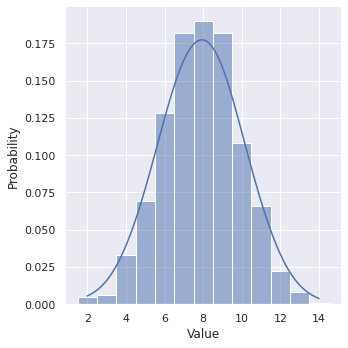
\includegraphics[width=\textwidth]{resources/task1_bin.png}
                \caption{Биномиальное распределение}
                \label{task1_bin}
            \end{subfigure}
            \hfill
            \begin{subfigure}[b]{0.5\textwidth}
                \centering
                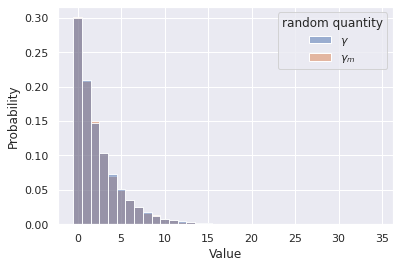
\includegraphics[width=\textwidth]{resources/task1_memo.png}
                \caption{Отсутствие памяти ($m = 5$)}
                \label{task1_memo}
            \end{subfigure}
            \caption{}
        \end{figure}


    \subsection{Игра в орлянку}
        Даны $n$ н.о.р.с.в.

        \[\theta_j: \mathbb{P}(\theta_j = 1 ) = \mathbb{P}(\theta_j = -1) 
                                          = \frac{1}{2}, \quad j = 1,\ldots,n.\]

        Рассматривается нормированная сумма

        \[Y(i) = \frac{S_i}{\sqrt{n}},\quad \text{где } 
                                       S_i = \sum\limits_{j = 1}^{n} \theta_j,\]

        пример поведения которой проиллюстрирован на рис. \ref{task1_toss}.

        \bigskip

        \begin{figure}[tbp]
            \centering
            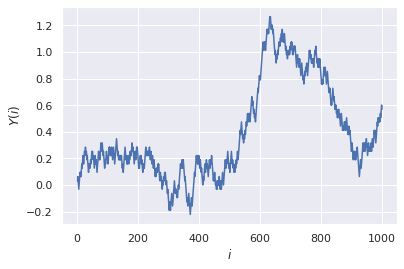
\includegraphics[width=0.5\textwidth]{resources/task1_toss.png}
            \caption{Игра в орлянку ($n = 1000$)}
            \label{task1_toss}
        \end{figure}

        Для оценки $Y(n)$ при $n \rightarrow \infty$, нам потребуется
        \begin{theorem}[Центральная предельная теорема]
            Пусть $\xi_1, \xi_2, \ldots$~--- последовательность независимых 
            одинаково распределенных (невырожденных) случайных величин с 
            $\Exp{\xi_1^2} \le \infty$ и $S_n = \xi_1 + \ldots + \xi_n$. Тогда
            \[\frac{S_n - \Exp{S_n}}{\sqrt{\Disp{S_n}}} 
            \stackrel{d}{\longrightarrow} \mathrm{Norm}(0,1).\]   
        \end{theorem}

        Действительно

        \[\frac{S_n - \Exp{S_n}}{\sqrt{\Disp{S_n}}} = 
        \frac{S_n - 0}{\sqrt{n\Disp{\theta_1)}}} = \frac{S_n}{\sqrt{n}} = Y(n) 
        \stackrel{d}{\longrightarrow} \mathrm{Norm}(0,1).\]
        